\chapter{Mercoledì 18/03/2020}
La scorsa volta abbiamo intodotto l'algebra relazionale per spiegare le procedure adottate dal DBMS per eseguire le nostre interrogazioni. Adesso analizzeremo la semantica effettiva del linguaggio: il calcolo relazionale. Sappiamo che in SQL non è necessario scrivere una query già ottimizzata: possiamo scrivere versioni meno efficienti che saranno sottoposte a un processo di ottimizzazione.

\section{Calcolo relazionale}
\noindent Con \textbf{calcolo relazionale} intendiamo una famiglia di linguaggi dichiarativi che permette di specificare le proprietà del risultato di una certa interrogazione. Ne abbiamo due versioni:
\begin{itemize}
	\item il calcolo relazionale \textbf{applicato ai domini} (che presenta in modo naturale le proprietà dei predicati)
	\item il calcolo \textbf{su tuple con dichiarazioni di range} (versione adottata da SQL)
\end{itemize}

\subsection{Calcolo su domini}
\[\{A_1: x_1, \dots, A_n : x_n | f \}\]
\begin{itemize}
	\item $A_1,\dots,A_n$ sono nomi di attributi, $x_1,\dots,x_n$ sono nomi di variabili
	\item La lista delle coppie $A_i:x_i$ è detta \emph{target list} e definisce la struttura del risultato
	\item $f$ è una formula. Al suo interno possiamo porre:
	\begin{itemize}
		\item $R(A_1:x_1,\dots,A_n:x_n)$, dove $R(A_1\dots A_n)$ è uno schema di relazione $x_1\dots x_n$ sono variabili. Vera sui valori $x_1,\dots,x_n$ che formano una tupla della relazione r sullo schema R, nell'istanza di base di dati a cui l'espressione viene applicata.
		\item $x\theta y$, $x\theta c$: $x,y$ sono variabili, $c\;$ è una costante e $\theta$ è un operatore di confronto ($=, \neq, \leq, \geq, >, <$). Vera sui valori $x,y,c$ che soddisfano il confronto con operatore $\theta$.
		\item quantificatori nella forma
		\[\exists x (f)\;\;\;\,\forall x (f)\]
		Cioè: \textit{Esiste almeno una variabile $x$ che soddisfa la formula $f$}
	\end{itemize}
	Se $f_1$ e $f_2$ sono formule allora lo sono anche $\neg f_1$, $\neg f_2$, $f_1 \land f_2$, $f_1 \lor f_2$.
\end{itemize}
\subsection{Calcolo su tuple con dichiarazione di range}
\[\{x_1.Z_1,\dots,x_n.Z_n | x_i(R_1),\dots,x_j(R_m) | f \}\]
\begin{itemize}
	\item $x_1.Z_1,\dots,x_n.Z_n$ è la \emph{target list} (con $x_i$ nome di tupla e $Z_j$ insieme di nomi di attributi)
	\item $x_i(R_1),\dots,x_j(R_m)$ è la \emph{range list} (campo di variabilità delle variabili)
	\item $f$ è una formula. Al suo interno possiamo porre:
	\begin{itemize}
		\item formule atomiche del tipo $x_i.Z_i \, \theta \, x_j.Z_j$ o $x_i.Z_i \, \theta \, c$ (dove $c$ è una costante).
		\item connettivi come nel calcolo su domini
		\item quantificatori nella seguente forma
		\[\exists x (R)(f)\;\;\;\;\;\forall x (R)(f)\]
		\small
		Cioè: \textit{Esiste nella relazione $R$ almeno una variabile $x$ che soddisfa la formula $f$}
		\normalsize
	\end{itemize}
\end{itemize}

\subsection{Quantificatori esistenziali e universali}
All'interno dei predicati possiamo introdurre i cosiddetti \emph{quantificatori}. Abbiamo il quantificatore esistenziale $\exists$ e quello universale $\forall$. I due sono intercambiabili, nel senso che ne basta uno per esprimere qualunque cosa. Le \emph{leggi di de Morgan} valgono, \emph{mutatis mutandis}, anche per i quantificatori:
\begin{itemize}
	\item $\exists x(f) = \neg(\forall x(\neg(f)))$
	\item $\forall x(f)=\neg(\exists x(\neg(f)))$
\end{itemize}
\paragraph{Ricordiamo le leggi di De Morgan, già viste a \emph{Fondamenti di programmazione}}
\[\boxed{\neg(f \land g)=\neg(f) \lor \neg(g)}\;\;\;\;\;\;\;\;\;\;\;\,\;\boxed{\neg(f\lor g) = \neg(f) \land \neg(g)}\]
Date due condizioni $f$ e $g$:
\begin{enumerate}
	\item La negazione dell'AND si ha quando almeno una delle condizioni è negata
	\item La negazione dell'OR si ha quando entrambe le condizioni sono negate
\end{enumerate}
\paragraph{Quando sono necessari?} I quantificatori possono essere omessi in certe circostanze, ma in altre sono obbligatori: parliamo di interrogazioni più complesse come, per esempio, la differenza.  

\subsection{Esempi}\paragraph{Base di dati per gli esempi}
\begin{Verbatim}[commandchars=+\[\]]
	IMPIEGATI(+underline[Matricola], Nome, Età, Stipendio)
	SUPERVISIONE(+underline[Capo, Impiegato])
\end{Verbatim}
\paragraph{Trovare gli impiegati che guadagnano più di 40 milioni} 
\begin{itemize}
	\item \textbf{Su domini}: \{ Matricola: m, Nome : n, Età: e, Stipendio: s $|$ Impiegati(Matricola: m, Nome: n, Età: e, Stipendio: s) $\land$ s $>$ 40 \}
	\item \textbf{Su tuple con dichiarazione di range}: \{i.* $|$ i(Impiegati) $|$ i.Stipendio $>$ 40\}
\end{itemize}
\paragraph{Trovare nome e matricola degli impiegati che guadagnano più di 40 milioni} 
\begin{itemize}
	\item \textbf{Su domini}: \{ Matricola: m, Nome: n $|$ Impiegati(Matricola: m, Nome: n, Età: e, Stipendio: s) $\land$ s $>$ 40\}
	\item \textbf{Su tuple con dichiarazione di range}: \{ i.(Matricola, Nome) $|$ i(Impiegati) $|$ i.Stipendio $>$ 40 \}
\end{itemize}
\paragraph{Trovare matricola e nome dei capi i cui impiegati guadagnano tutti più di 40 milioni}
\begin{itemize}
	\item \textbf{Primo metodo con calcolo sui domini}: \{ Matricola: c, Nome: n $|$ Impiegati(Matricola: c, Nome: n, Età: e, Stipendio: s) $\land$ $\forall m'(\forall n' (\forall e' ( \forall s'(Impiegati$(Matricola: m', Nome: n', Età: e', Stipendio: s'\} $\land$ Supervisione(Capo:c, Impiegato:m') $\land$ s' $>$ 40))))\}
	\item \textbf{Secondo metodo con calcolo sui domini}: \{ Matricola: c, Nome: n $|$ Impiegati(Matricola: c, Nome: n, Età: e, Stipendio: s) $\land$ $\neg(\exists m'(\exists n' (\exists e' ( \exists s'(Impiegati$(Matricola: m', Nome: n', Età: e', Stipendio: s'\} $\land$ Supervisione(Capo:c, Impiegato:m') $\land$ s' $\leq$ 40)))))\}
	\item \textbf{Terzo metodo con calcolo su tuple}: \{i.(Matricola, Nome) $|$ s(Supervisione), i(Impiegati) $|$ i.Matricola = s.Capo $\land$ $\neg(\exists i$(Impiegati)(s.Impiegato=i.Matricola $\land$ i.Stipendio $\leq$ 40)))\}
\end{itemize}
\subsection{Discussione sul calcolo su domini}
Il calcolo su domini è dichiarativo, ma eccessivamente verboso con possibilità di scrivere espressioni sensa senso dipendenti dal dominio e aventi risultati di grandi dimensione. Nell'algebra, invece, tutte le espressioni hanno un senso e sono indipendenti dal dominio.
\paragraph{Indipendenza dal dominio} Un'espressione si dice indipendente dal dominio se il suo risultato, su ciascuna istanza di base di dati, non varia al variare del dominio rispetto al quale l'espressione è valutata.
\paragraph{Esempio di espressione dipendente dal dominio} Un esempio di espressione dipendente dal dominio è la seguente:
\[\{ A_1 : x_1, A_2 : x_2\;|\;R(A_1 : x_1, A_2 : x_2) \land x_2 = x_2 \}\]
$x_2 = x_2$ è una condizione sempre vera: se il dominio include gli interi da $0$ a $99$ avremo 100 tuple, se invece il dominio va da $0$ a $999$ avremo 1000 tuple!
\subsection{Discussione sul calcolo su tuple}
Le variabili rappresentano tuple e si ha minore verbosità. Alcune interrogazioni importanti non possono essere espresse, in particolare le unioni:
\[R_1(AB) \cup R_2(AB)\]
Ogni variabile nel risultato ha un solo range, mentre vorremmo tuple sia della prima relazione che della seconda. Intersezione e differenza, comunque sia, sono esprimibili. Per questa motivazione SQL prevede esplicitamente un operatore unione, ma non tutte le versioni prevedono intersezione e differenza.
\subsection{Calcolo e algebra relazionale}
Calcolo e algebra relazionale sono ''equivalenti'':
\begin{itemize}
	\item Per ogni espressione del calcolo relazionale che sia indipendente dal dominio esiste un'espressione dell'algebra relazionale equivalente a essa
	\item Per ogni espressione dell'algebra relazionale esiste un'espressione del calcolo relazionale equivalente a essa (e di conseguenza indipendente dal dominio)
\end{itemize}
Possono espresse buona parte delle interrogazioni, però ci sono cose non esprimibili come la \emph{chiusura transitiva}.
\subsection{Chiusura transitiva di una relazione}
La chiusura transitiva non può essere definita poichè dovrei fare il JOIN innumerevoli volte per arrivare al risultato, alla tabella definitiva.
\paragraph{Esempio} Consideriamo la seguente relazione
\begin{Verbatim}[commandchars=+\[\]]
	Supervisione(+underline[Impiegato, Capo])
\end{Verbatim}
Voglio trovare, per ogni impiegato, tutti i superiori (cioè il capo, il capo del capo, e così via). Nel seguente esempio (teniamo conto che vi è la ridenominazione dell'attributo \emph{Campo}) la cosa pare semplice
\begin{center}
	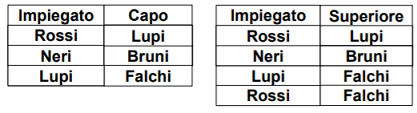
\includegraphics{images/140.PNG}
\end{center}
ma se abbiamo una nuova n-upla come nel secondo esempio risulta necessario stabilire ulteriori legami. Se il capo di Rossi è Lupi e il capo di Lupi è Falchi allora il capo di Rossi è Falchi.
\begin{center}
	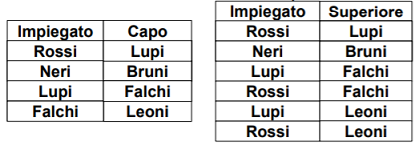
\includegraphics{images/141.PNG}
\end{center}
\paragraph{Conclusione} Non possiamo calcolare la chiusura transitiva di una relazione qualunque. In algebra relazionale l'operazione si simulerebbe con un numero di JOIN illimitato.

\section{Estensione dell'algebra relazionale}
Il modello relazionale può essere facilmente estesso a comprendere operatori SQL non direttamente riconducibili agli operatori algebrici introdotti. Ciò non comporta una modifica del modello.
\subsection{JOIN Esterno}
Ho tre tipi di OUTER JOIN: left, right e full. Questi permettono di combinare tuple che normalmente non fanno JOIN.
\begin{itemize}
	\item Il LEFT JOIN: mantiene tutte le tuple della prima relazione
	\item Il RIGHT OUTER JOIN: mantiene tutte le tuple della seconda relazione
	\item Il FULL OUTER JOIN: mantiene tutte le tuple
\end{itemize}
\paragraph{Esempio di JOIN} \emph{Trovare la matricola dei capi degli impiegati che guadagnano tutti più di 40.000 euro}
\begin{center}
	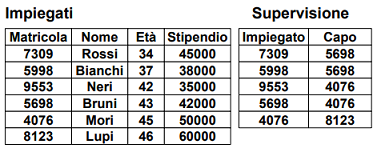
\includegraphics{images/60.PNG}
\end{center}
Si individuano impiegati non subordinati a nessuno, cioè i capi stessi. Con un JOIN normale (con I.Matricola e S.Impiegato) i record riguardanti questi impiegati sparirebbero. Facciamo il JOIN sinistro
\[\pi_{Capo}(\sigma_{Matricola IS NULL}(Supervisione = \Join_{Impiegato=Matricola} \sigma_{Stipendio \leq 40.000}(Impiegati)))\]
ottenendo
\begin{center}
	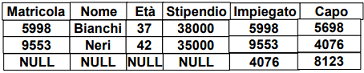
\includegraphics{images/61.PNG}
\end{center}
Ho due impiegati che soddisfano le condizioni e un capo che non ha impiegati che guadagnano più di 40.000 euro. Ho tuple che fanno JOIN e tuple che non hanno fatto JOIN. Quanto fatto permette di svolgere l'operazione di differenza, che vedremo più avanti
\subsection{Proiezione generalizzata}
\[\pi_{F_1,F_2,F_3}(E)\]
Dove $F_1,F_2,F_3$ sono espressioni aritmetiche su attributi di $E$ e costanti. Creo "un nuovo" attributo derivante da un'espressione algebrica dipendente da altri attributi e da costanti. Vediamo un esempio con la seguente tabella
\begin{center}
	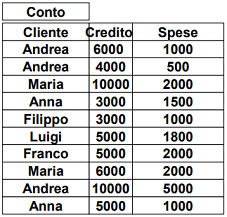
\includegraphics{images/62.PNG}
\end{center}
Posso scrivere, per esempio $\pi_{Cliente,Credito-Spese}(Conto)$, ottenendo
\begin{center}
	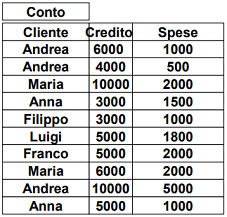
\includegraphics{images/62.PNG}
\end{center}
\subsection{Funzioni aggregate}
Si possono usare nelle espressioni dei nomi di funzione (operatori) che si applicano a insiemi e producono un valore scalare come risultato. Gli operatori aggregati sono:
\begin{itemize}
	\item \textbf{Somma}: $sum_{Spese}(Conto)$
	\item \textbf{Massimo}: $max_{Credito}(Conto)$
	\item \textbf{Minimo}: $min_{Credito}(Conto)$
	\item \textbf{Conteggio}: $count_{Cliente}(Conto)$
	\item \textbf{Conteggio di elementi distinti}: count-distinct$_{Cliente}(Conto)$
\end{itemize}
\subsection{Raggruppamento}
Posso raggruppare gli elementi di una relazione attraverso un apposito operatore. Posso raggruppare dei conti in base al codice cliente ravvicinando i conti correnti dei vari clienti. Posso applicare a questi gruppi degli operatori aggregati e ottenere un result set con una riga per ogni cliente.
\[_\mathbf{Cliente}G_{sum(Credito)}(Conto)\]
Posso avere più attributi con cui compiere il raggruppamento (a sinistra), ma anche più funzioni di aggregazione (a destra).
\subsection{Divisione}\footnote{Sezione da imparare come l'ave maria. La Vaglini chiede molto spesso di spiegare la divisione. Ringrazio Giovanni Ligato per avermi spiegato la cosa il giorno prima dell'orale (mi ha letteralmente salvato la vita).}
Operatore di tipo universale (parola chiave: tutti). Posso porlo sintatticamente all'interno di una query, ovviamente non è primitivo perchè corrisponde a un'espressione estremamente complessa.
\paragraph{Esempio} \emph{Trovare i nomi dei clienti che hanno un conto corrente in tutte le filiali di banca di Pisa}.\\Abbiamo le seguenti relazioni:
\begin{Verbatim}[commandchars=+\[\]]
	Branch(+underline[bank_name,branch_name], branch_city)
	Account(branch_name, bank_name, +underline[account_number], branch_city)
	Depositor(+underline[account_number], customer_name)
\end{Verbatim}
Possiamo risolvere l'esercizio attraverso la seguente espressione algebrica:
\[\Pi_{CN,BrN}(depositor \Join account) \div \Pi_{BrN}(\sigma_{BC='Pisa'}(branch))\]
Il risultato sono i clienti che hanno un conto in tutte le filiali di Pisa. L'espressione precedente, derivata, corrisponde alla seguente
\begin{align*}\Pi_{CN}(depositor \Join \sigma_{BC='Pisa'}(account)) - \Pi_{CN}(\\((\Pi_{CN}(depositor\Join \sigma_{BC='Pisa}(account)) \Join \Pi_{BrN}(\sigma_{BC='Pisa}(branch))\\-\\\Pi_{CN,BrN}(depositor \Join account)\\)\end{align*}
\begin{itemize}
	\item Prendo i clienti che esistono e hanno almeno un conto in una filiale di Pisa. 
	\item Attraverso un prodotto cartesiano (osservo dalle proiezioni che non metto insieme tuple con attributi comuni) genero tutte le coppie possibili tra i clienti che hanno conti a Pisa e le sedi di Pisa. Il risultato intermedio è caratterizzato da coppie veritiere (coloro che hanno effettivamente un conto in quella sede) e coppie false (persone che non hanno un conto in quella sede)
	\item Da questo prodotto cartesiano sottraggo le coppie veritiere (tutte, incluse quelle non di Pisa)
	\item La differenza più esterna mi porta ad ottenere coloro che hanno conti solo a Pisa.
	\item \textbf{Persona che ha conti solo a Pisa}: le coppie ottenute attraverso il prodotto cartesiano sono tutte veritiere. Segue che la differenza più interna le rimuoverà. Quindi la differenza più esterna non mi va a rimuovere questa persona.
	\item \textbf{Persona che non ha conti in tutte le filiali di Pisa}: le coppie ottenute attraverso il prodotto cartesiano sono in parte veritiere e in parte false. Attraverso la differenza più interna rimuovo le coppie veritiere. Mi rimangono le coppie false. Se ci sono coppie false significa che l'utente non ha conti in tutte le filiali di Pisa
\end{itemize}
%\paragraph{Quindi} La divisione consiste in una relazione su $R-S$. Date $r(R)$ e $s(S)$, con $R$ che contiene $S$, una tupla $t$ appartenente alla relazione divisione presenta le seguenti proprietà
%\begin{itemize}
%\item $t \in \Pi_{R-S}(r)$ (proiezione degli attributi della relazione $R-S$)
%\item $\forall t' \in s, \exists t'' \in r$ tale che
%\begin{itemize}
%\item $t'[S]=t''[S]$
%\item $t'[R-S]=t$
%\end{itemize}
%Per ogni tupla appartenente alla relazione $s$ esiste un'altra tupla appartenente alla relazione $r$ che sono uguali, con la proiezione degli attributi $S$. La seconda tupla, con gli attributi di $R-S$ è uguale a una tupla appartenente $\pi_{R-S}(r)$.
%\end{itemize}
\section{Relazioni derivate}
\paragraph{Relazioni di base} Presentano un contenuto autonomo
\paragraph{Relazioni derivate} Relazioni il cui contenuto è funzione del contenuto di altre relazioni. Quando compiamo un'interrogazione costruiamo dei risultati intermedi senza intaccare la base di dati. Potrei avere il bisogno di recuperare un risultato (anche più di una volta) assegnandogli un nome. Ciò consiste in una \emph{vista}. Essa può essere materializzata (salvata e usata più volte) o virtuale (usata una volta sola).
\begin{itemize}
	\item \textbf{Viste materializzate}: La memorizzazione risulta vantaggiosa perchè non hai da fare il calcolo tutte le volte (si hanno delle tabelle in carne ed ossa, ripensare a quanto visto con Pistolesi). I risultati sono immediatamente disponibili, ma potrebbero essere ridondanti e appesantire. Le viste materializzate non sono supportate da tutti i DBMS
	\item \textbf{Viste virtuali}: La vista virtuale è sempre ricalcolata ed è supportata da tutti i DBMS (nel db salviamo non il result set, ma lo snippet - il testo dell'interrogazione).
\end{itemize}
\paragraph{Colleghiamo a quanto fatto fino ad ora} Ottenere una vista significare dare un nome a un espressione. Esempio:
\[Supervisione = \pi_{Impiegato,Capo}(Afferenza \Join Direzione)\]
Posso adottare questa vista anche in altre espressioni:
\[\sigma_{Capo='Leoni'}(Supervisioni)\]
viene eseguita come
\[\sigma_{Capo='Leoni'}(\pi_{Impiegato,Capo}(Afferenza \Join Direzione))\]
\paragraph{Vantaggi per il programmatore} Possiamo semplificare la scrittura di interrogazioni seguendo il metodo del \emph{divide et impera} (divisione di un problema in sottoproblemi)